% ==============================================================================
% TCC - Nome do Aluno
% Capítulo 3 - Especificação de Requisitos
% ==============================================================================
\chapter{Algoritmo A*}
\label{sec-aestrela}

\section{O Algoritmo}
\label{sec-aestrela-algoritmo}
O algoritmo A* (lê-se "A estrela"), também conhecido como busca A*, é um algoritmo de busca informada em grafos. Foi proposta originalmente em \citeonline{hart1968formal} e pode ser visto como uma adaptação do algoritmo de Dijkstra (apresentado no capítulo \ref{sec-dijkstra}) em que, ao invés de se calcular a melhor rota de um ponto de partida para todos os demais vértices do grafo, se estabelece uma boa rota (ou mesmo a rota ótima\footnote{A garantia do valor ótimo do algoritmo depende de fatores que serão discutidos na subseção \ref{sec-aestrela-algoritmo-heuristica}.}) partindo do vértice origem a um vértice destino. Isso é feito realizando "podas" do caminho de forma que não seja necessário visitar todos os vértices, apenas os mais promissores do grafo.

A seguir é apresentado o algoritmo A* adaptado de \citeonline{likhachev2008anytime} sobre o algoritmo de Dijkstra apresentado na seção \ref{sec-dijkstra-algoritmo}. 

\begin{lstlisting}[ mathescape, label=lst-aestrela-codigo, caption=Algoritmo A*, float=htpb]
$A^{*}$Algorithm(weighted simple digraph, vertex first, vertex goal)
	for all vertices v
		g(v) = $\infty$;
	g(first) = 0;
	toBeChecked = all vertices;
	while goal is in toBeChecked
		v = a vertex in toBeChecked with minimal f(v);
		remove v from toBeChecked;
		for all vertices u adjacent to v and in toBeChecked
			if g( u ) > g( v ) + weight( edge(vu) )
				g( u ) = g( v ) + weight( edge(vu) );
				predecessor( u ) = v;
				update u in toBeChecked with f(u) = g(u) + h(u);
\end{lstlisting}

O algoritmo segue em sua essência como um Dijkstra adaptado. Iniciamos a distância de todos os vértices g(v) (valor que corresponde ao valor da distância calculada do vértice origem "first" até o vértice "v") como sendo $\infty$\footnote{Vide nota de rodapé da seção \ref{sec-dijkstra-algoritmo}.}, com exceção do vértice origem, cujo valor atribuído é zero. Adicionamos todos os vértices ao grupo "toBeChecked" \footnote{Algumas literaturas designam esse conjunto como OPEN.}. Feito isso inicia-se o processo iterativo: enquanto o vértice "goal" estiver dentro do conjunto "toBeChecked" (ou seja, o vértice "goal" não foi alcançado ainda), o vértice com menor valor f(v) é retirado do conjunto "toBeChecked" e para cada vértice adjacente u de v, verifica-se se o valor de g( u ) atual é maior que g( v ) mais o peso da aresta entre v e u (edge(vu)). Em caso afirmativo, o valor de g( u ) é atualizado para g( v ) mais o peso da aresta entre v e u, e v é marcado como o predecessor de u. O valor do peso do vértice u é atualizado na fila de prioridades utilizada (como a heap binária, descrita na subseção \ref{sec-dijkstra-versoes-heap}) com o valor f( u ) = g( u ) + h( u ).

Observe que para o algoritmo A*, diferente do que ocorre em Dijkstra, não se utiliza o valor de g( u ) (valor da distância calculada do vértice origem "first" até o vértice "u") como chave de ordenamento da fila de prioridade, mas sim esse valor acrescido de h( u ). Observe também que o algoritmo termina ao ser removido o vértice destino ("goal") da lista do "toBeChecked" em contrapartida ao Dijkstra que calcula as distâncias para todos os vértices do grafo. O termo h( u ) consiste no valor heurístico que corresponde a uma estimativa da distância de u ao vértice destino "goal". É devido a esse valor que o algoritmo A* realiza "podas" no número de vértices a serem checados, buscando os mais promissores, já que esse valor faz com que os vértices cujas estimativas sejam mais próximas do vértice destino ("goal") sejam colocados mais a frente na fila de prioridades e por consequência, sejam calculados primeiro. E assim é mais provável que o vértice destino seja alcançado antes e tenha sua rota calculada, terminando o algoritmo. O valor h( u ) é classificado como admissível e não-admissível cujo significado será discutido na subseção \ref{sec-aestrela-algoritmo-heuristica}.

A figura \ref{fig-aestrela-algoritmo-mapa1} contida em \citeonline{russell1995modern} mostra um exemplo de aplicação do algoritmo.

\begin{figure}[H]
\centering
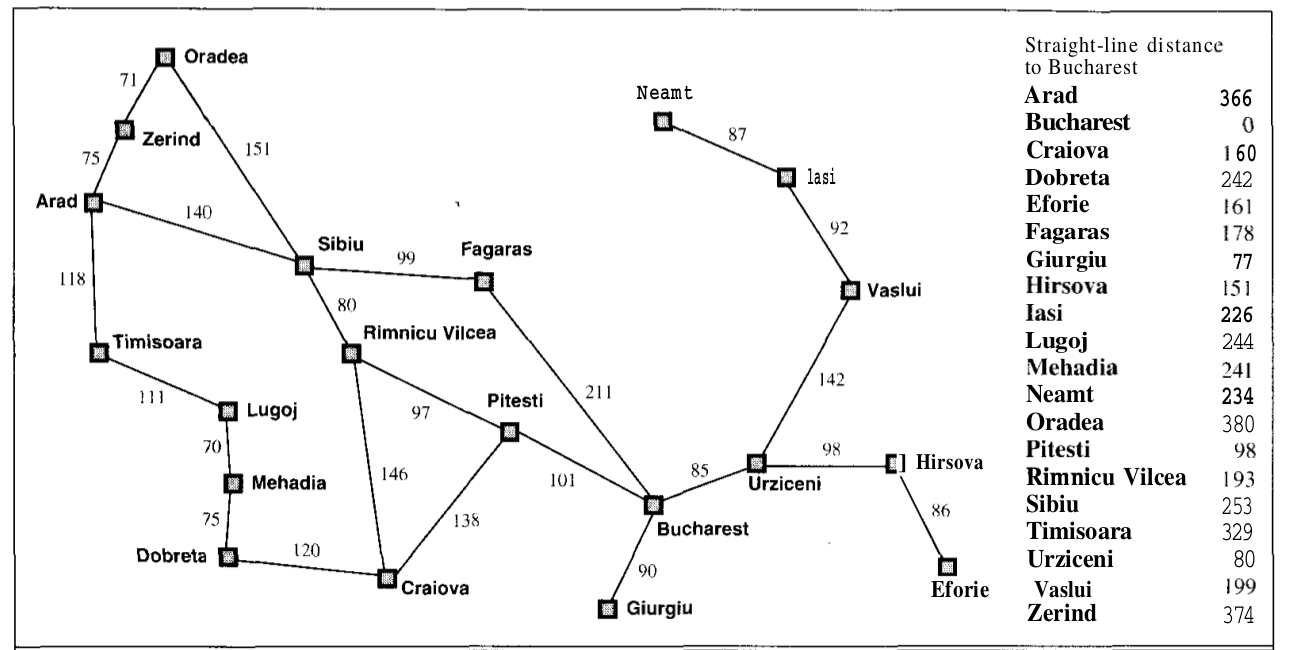
\includegraphics[width=.90\textwidth]{figuras/Aestrela-mapa1} 
\caption{Mapa da Romênia com os valores das distâncias entre as cidades e a distância euclidiana de todas elas até Bucareste.}
\label{fig-aestrela-algoritmo-mapa1}
\end{figure}

Um viajante deseja partir da cidade de Arad com destino a Bucareste buscando percorrer o menor caminho entre essas duas cidades. Para isso é utilizado o algoritmo A* que explora o grafo conforme descrito na figura \ref{fig-aestrela-algoritmo-mapa2}\footnote{A figura \ref{fig-aestrela-algoritmo-mapa2} foi obtida do vídeo "Algoritmo A*" contido no sítio eletrônico \url{https://www.youtube.com/watch?v=6CqZ5AaTfhQ}, acesso em 25 de abril de 2017.}, tendo como heurística utilizada, a distância euclidiana entre todas as cidades e Bucareste (distâncias também representadas na figura \ref{fig-aestrela-algoritmo-mapa1}).

\begin{figure}[H]
\centering
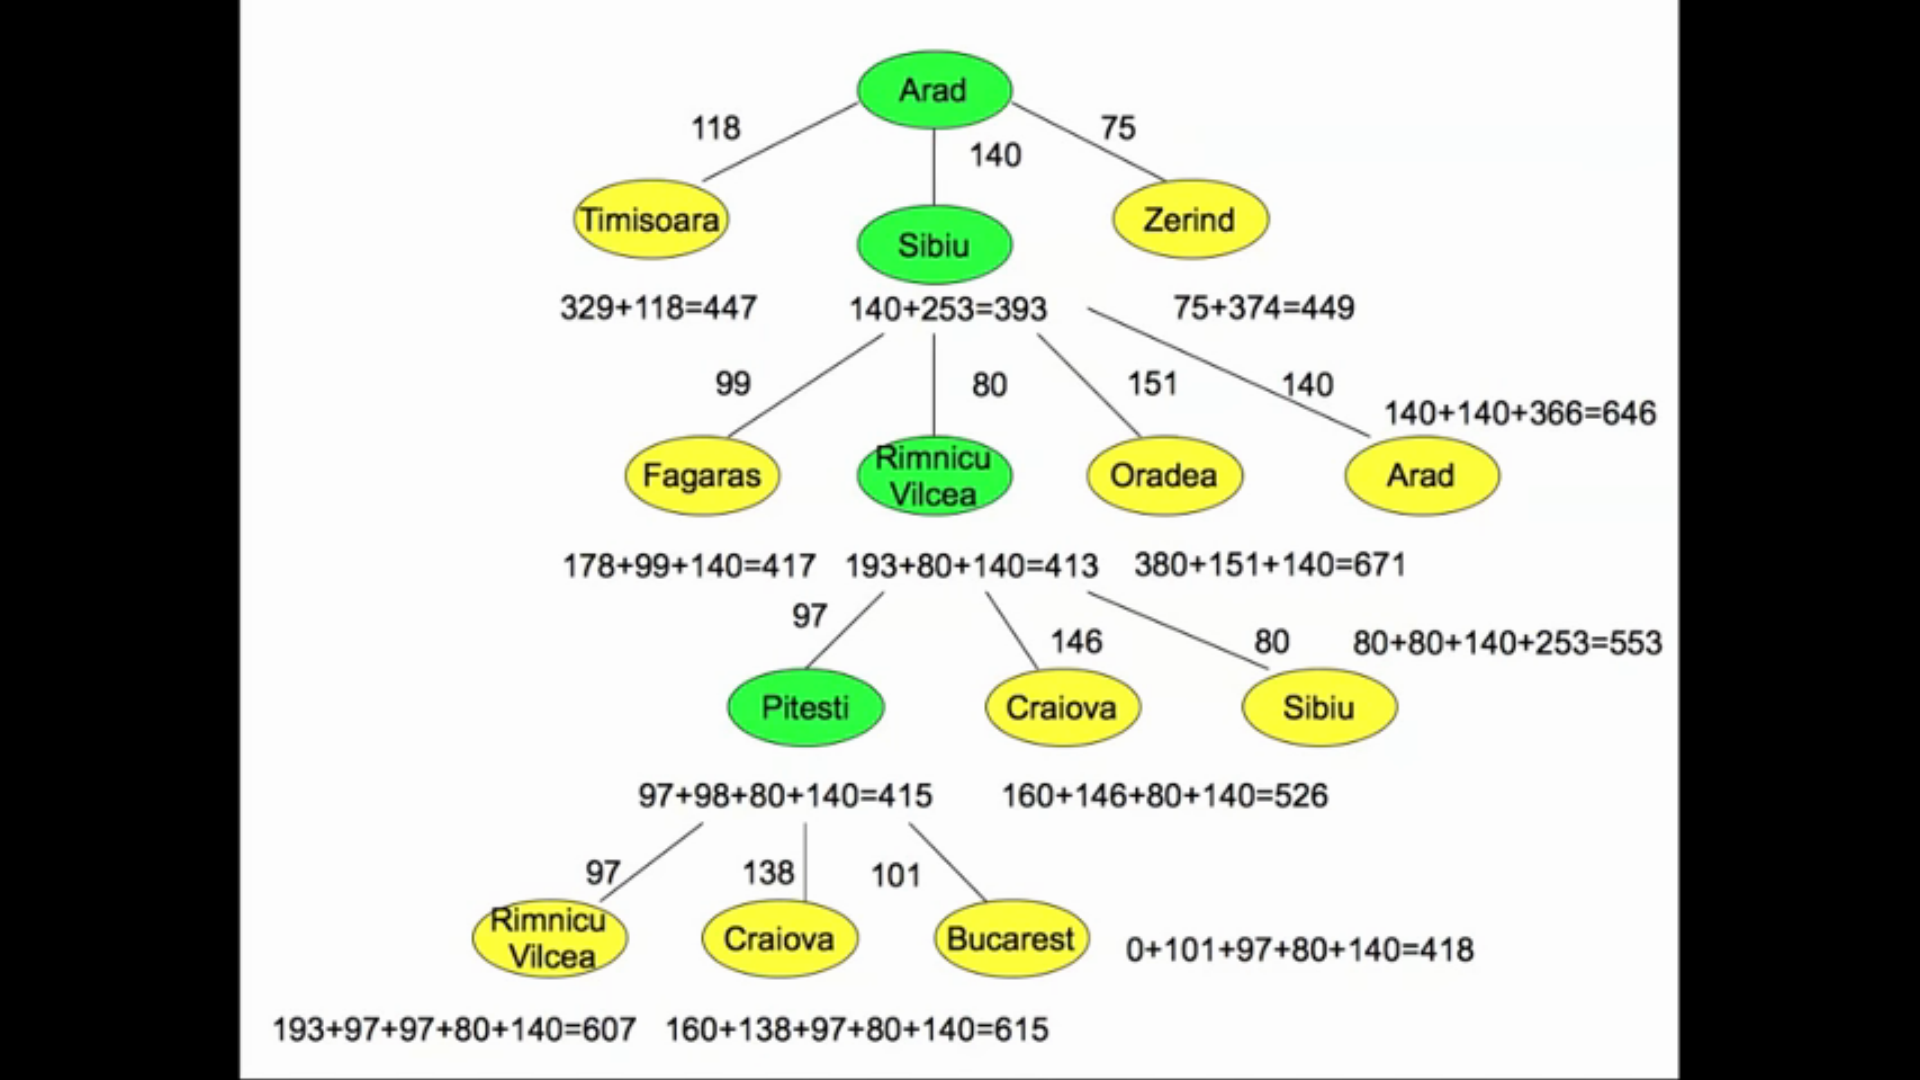
\includegraphics[width=.90\textwidth]{figuras/Aestrela-mapa2} 
\caption{Desenvolvimento do algoritmo A*.}
\label{fig-aestrela-algoritmo-mapa2}
\end{figure}

O procedimento é bem semelhante ao de Dijkstra (descrito no capítulo \ref{sec-dijkstra}), inicialmente é atribuído o valor de distância de todos os vértices g(v) como $\infty$, com exceção do vértice de origem que é atribuído como zero. Neste exemplo da figura \ref{fig-aestrela-algoritmo-mapa2}, o vértice de origem é a cidade de "Arad". Dela se expande para seus vértices vizinhos, que no caso são as cidades de "Timisoara", "Sibiu" e "Zerind". A fila de prioridades é atualizado conforme a função f( u ) = g( u ) + h( u ). Sendo assim o próximo vértice a ser explorado é a cidade de "Sibiu". Vemos o fator heurístico "pesando" na escolha do próximo vértice a ser escolhido, pois por Dijkstra, o próximo vértice a ser escolhido seria "Zerind", ao invés de "Sibiu", pois aquela possui aresta com peso menor do que esta. Dela se expande para as cidades vizinhas de "Fagaras", "Rimnicu Vilcea" e "Oradea". "Rimnicu Vilcea" é tida a cidade mais promissora e dela continua a expansão para as suas cidades vizinhas de "Pitesti", "Craiaova" e "Sibiu". "Pitesti" é escolhida. E dela se expande para as suas cidades vizinhas de "Rimnicu Vilcea", "Craiova" e finalmente "Bucarest" que é a cidade destino e que tem fator heurístico igual a zero, sendo portanto mais provável a sua escolha na próxima iteração, terminando assim o algoritmo. \textbf{[A REVISAR]}


%\citeonline{russell1995modern,cormen2009introduction}.

%\begin{lstlisting}[ mathescape, label=lst-aestrela-codigo, caption=Algoritmo A*, float=htpb]
%Entrada: Grafo G, vértice inicial $v_{i}$, vértice destino $v_{f}$
%	para todo vértice $s \in V(G), s \neq vi$ faça
%		$g(s) = \infty$
%	fim para
%	$g(v_{i}) = 0$
%	para todo vértice $s \in V(G)$ faça
%		anterior($s$) = -1
%	fimpara
%	OPEN = {$v_{i}$}
%	enquanto $v_{f}$ não é expandido faça
%		s = desenfila(OPEN)
%		para cada sucessor $s'$ de $s$ faça
%			se $g(s') > g(s) + c(s,s')$ então
%				$g(s') = g(s) + c(s,s')$
%				anterior($s'$) = s
%				insira/atualize $s'$ em OPEN pelo valor de f
%			fim se
%		fim para
%	fim enquanto
%retorna anterior
%\end{lstlisting}



\subsection{Heurísticas admissíveis e não-admissíveis}
\label{sec-aestrela-algoritmo-heuristica}  
O fator heurístico h( u ) é uma estimativa da distância entre o vértice "u" e o vértice "goal". Ela é chamada de \textbf{admissível} quando o valor da estimativa garantidamente não superestima o valor da distância real entre "u" e "goal" \cite{russell1995modern}. Um exemplo clássico usado de heurística admissível é a distância euclidiana, já que a menor distância entre dois pontos é uma reta \cite{russell1995modern}.

O cálculo da distância euclidiana porém, nem sempre é a forma mais rápida em termos computacionais, já que geralmente ela é calculada em termos dos pontos geográficos do vértice e esse cálculo envolve exponenciação e radiação. É por isso que existe o uso de heurísticas \textbf{não-admissíveis} que são estimativas que visam a usar cálculos mais simples e que, porém, não há a garantia que essa distância superestime a distância real entre "u" e "goal". Por consequência não há garantia que o caminho ótimo seja encontrado.

Exemplos de heurísticas não-admissíveis:
\begin{itemize}
\item Distância Manhattan:
\begin{itemize}
\item h( u ) = $| x_{u} - x_{goal} | + | y_{u} - y_{goal}|$;
\end{itemize}
\item Atalho Diagonal:
\begin{itemize}
\item h( u ) = $\sqrt{2} * | y_{u} - y_{goal}| + ( | x_{u} - x_{goal} | - | y_{u} - y_{goal}| )$ [Se a distância $| x_{u} - x_{goal} | > | y_{u} - y_{goal}|$];
\item h( u) = $\sqrt{2} * | x_{u} - x_{goal}| + ( | y_{u} - y_{goal}| - | x_{u} - x_{goal} | )$ [Se a distância $| x_{u} - x_{goal} | < | y_{u} - y_{goal}|$];
\end{itemize}
\end{itemize}